\chapter{History of Neural Networks}\label{ch_history}
\chapterauthor{Jeff Yoshimi, Pierre Beckmann}{.95, .05}

% Consider separating second winter, and deep learning resurgence, even if the resulting sections are short, for a cleaner presentation.
% Can say more about the two resurgences.  Both involves more on learning intermediate reps in FF networks. Part of a narrative across chapters
% Add AI Winter and Lighthill as contemporaneous
% Add more explicit discussion of neobehaviorism and Clark Hull (search Hull below)

This chapter briefly outlines the history of neural networks, including the pre-history of neural networks and cognitive science extending back to ancient Egypt. The theory of neural networks has many historical precedents, but emerged as an explicit mathematical and computational formalism in the mid 1900s, via the work of McCulloch and Pitts. The main events developed in the chapter are shown in Fig. \ref{timelineHistory}. 

\begin{figure}[h]
\centering
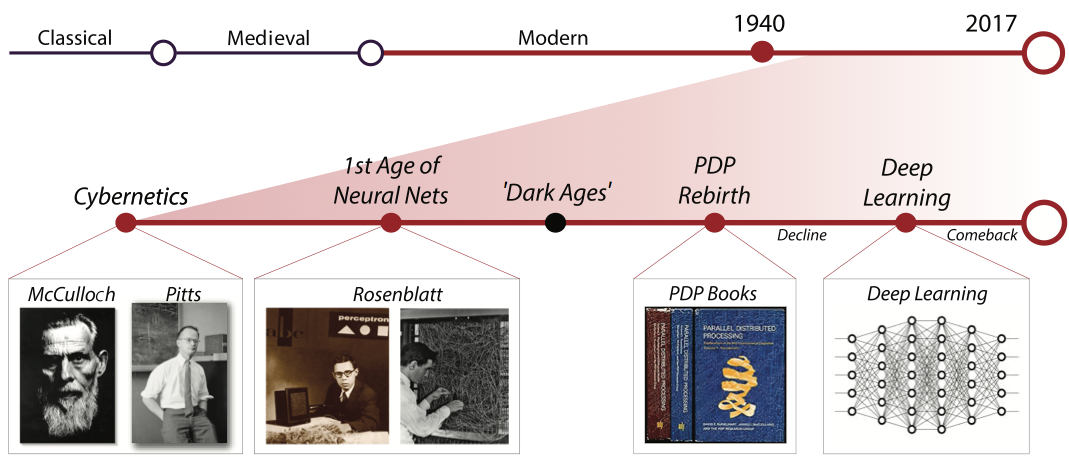
\includegraphics[width=0.8\textwidth]{images/historyTimeline.png}
\caption[Pamela Payne and Jeff Yoshimi.]{A timeline of the history of neural networks. The main history of neural networks runs from the mid 1940s to the present. We  also consider some of the pre-history of neural networks,  i.e. historical figures who linked the structure and dynamics of the mind with the structure and dynamics of the brain.}
\label{timelineHistory}
\end{figure}
% Black dot for second decline to match first

\section{Pre-history}

Cognitive science, the interdisciplinary study of mind, has ancient roots. Documentation of the idea that the brain plays some role in controlling behavior goes back to an Egyptian papyrus that is over 3000 years old.\footnote{The papyrus can be viewed online; try searching for ``Smith papyrus''. Recent scholarship on the papyrus is collected in \cite{meltzer2014edwin}.} Hieroglyphics from the papyrus describing the gyrations of the brain are shown in Fig. \ref{papyrus}. 
% Source: https://www.princeton.edu/~cggross/Hist_Neurosci_Ency_neurosci.pdf

\begin{figure}[h]
\centering

\includegraphics[width=0.4\textwidth]{images/papyrus.png}
\caption[From \url{https://faculty.washington.edu/chudler/papy.html}]{Hieroglyphics describing the sulci and gyri of the brain.}
\label{papyrus}
\end{figure}

In Western philosophy and science, Plato, Aristotle, and other Greek philosophers had an interest in the structure of the human mind (or ``soul'') in relation to physical processes in the body.\footnote{I focus on Western roots of neural network theory, though there were precedents in other parts of the world, which I hope to add in future versions of this chapter. Currently, the literature is sparse. There is an expanding literature on the history of science globally (e.g \cite{selin2013encyclopaedia}), but there is not (as of 2017) much scholarship on the history of neuroscience, cognitive science, or psychology in Africa, Asia, India, Mesoamerica, the Middle East, and other regions whose historical documents contain relevant information. There is however, some literature on  Arabic and Islamic roots of neuroscience \cite{mohamed2008arab}.}  Plato and Aristotle both described the soul as a set of interacting faculties (in Plato: reason, spirit, and appetite), and both speculated about its physical basis. They disagreed  about whether the brain or heart is the physical basis of the soul (Aristotle thought the brain just cooled the blood), but by the end of the Classical period the dispute was resolved in favor of the brain \cite{finger2001origins}.

In the Medieval period, priests, physicians, and natural philosophers throughout Europe and the Middle East discussed cognition in relation to the brain. Cognition was thought to be based on the play of ``spirits'' or vapors in the ventricles of the brain \cite{finger2001origins}. Spirits originating in the senses were combined in the ``common sense'' and then purified, and mixed in higher ventricles. A typical diagram from the period is shown in figure \ref{medieval}. The ventricles are now believed to be shock-absorbers and chemical reservoirs. They are not thought to play a central functional role in cognition. However, the idea that sensory inputs to the brain are combined and refined in various ways persists in connectionist models.
% https://web.stanford.edu/class/history13/earlysciencelab/body/brainpages/brain.html   // Mention Avicenna here
% One of the animal internal faculties of perception is the faculty of fantasy, i.e., sensus communis, located in the forepart of the front ventricle of the brain. It receives all the forms which are imprinted on the five [external] senses and transmitted to it from them. Next is the faculty of representation located at the rear part of the front ventricle of the brain, which preserves what the sensus communis has received from the five senses even in the absence of the sensed object. … Next is the faculty of the 'sensitive imagination' in relation to the animal soul, and the 'rational imagination' in relation to the human soul. This faculty is located in the middle ventricle of the brain near the vermiform process, and its function is to combine certain things with others in the faculty of representation, and to separate some things from others as it chooses. Then there is the estimative faculty located in the far end of the middle ventricle of the brain, which perceives the non-sensible intentions that exist in the individual sensible objects, like the faculty that judges that the wolf is to be avoided and the child is to be loved. Next there is the retentive and recollective faculty located in the rear ventricle of the brain, which retains what the estimative faculty perceives of the non-sensible intentions existing in individual sensible objects. (Avicenna, translated in Rahman 1952, p. 31)
% https://www.acsu.buffalo.edu/~duchan/new_history/middle_ages/ventricular_theory.html


\begin{figure}[h]
\centering
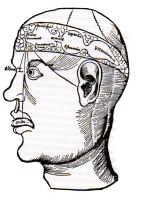
\includegraphics[width=0.2\textwidth]{./images/humoral.png}
\caption[From Gr\"{u}sser, 1990 \cite{grusser1990seat}]{A medieval diagram which shows how spirits were thought to flow and combine through the ventricles of the brain. Different ventricles were associated with different faculties, such as sensation and the ``common sense,'' integrating different senses, imagination, memory, and reason.}
\label{medieval}
\end{figure}

%Descartes?
During the Enlightenment, many speculated that connections between ideas in the mind are based on connections between fibers in the brain (neurons had not yet been identified as distinct structures.)\footnote{For more on this period of history, see Sutton (1998) \cite{sutton1998philosophy}. Sutton's discussion of Descartes is especially interesting, since it shows how Descartes had a connectionist styled account of the brain, which on his view  interacts with a non-physical soul via patterns of activity at the pineal gland. Other mechanist philosophers of the period such as Hobbes and La Mettrie had similar accounts but rejected the assumption of a non-physical soul.} In the 1700s, the empiricists Locke, Berkeley, and Hume famously claimed that ideas in the mind result from associations between simple sensory ideas: for example, a percept of an apple is composed out simple sensations corresponding to its color, shape, smell, and taste. One idea comes to mind, it calls another to mind, etc. Sometimes this happens instantaneously, as in the apple percept, but in other cases it might unfold in a temporal progression. Someone mentions apples, and that might make you think of fiber, which might in turn make you think of Raisin Bran. If someone mentions a person you know, associated thoughts about them--their age, where they live, their occupation, physical appearance, etc.--might also come to mind. One idea comes to mind, it calls another to mind, etc. Thus, the empiricists thought of the mind as something like an Interactive Activation and Competition (IAC) network (cf. Chapter \extref{ch_intro}) \cite{bain1873mind}.

In this period, David Hartley argued that the empiricist theory of associations could be explained by laws governing connected neurons \cite{hartley1834observations, bain1873mind}. For example, Hartley \cite{hartley1749observations} proposed that sensations $A,B,C,...$ which are associated with each other, are associated because of correlated associations between ``vibrations'' of brain fibers:
\begin{quotation}
PROPOSITION 10: Any sensations $A, B, C$, etc., by being associated with one another a sufficient number of times get such a  power over the corresponding ideas $a, b, c$ etc., that any one of the sensations $A$, when impressed alone, shall be able to excite in the mind $b, c,$ etc., the ideas of the rest.

PROPOSITION 11: Any vibrations $A, B, C,$ etc., by being associated with one another a sufficient number of times get such a  power over the corresponding miniature vibrations $a, b, c$ etc., that any one of the vibrations $A$, when excited alone, shall be able to excite in the mind $b, c$, etc. 
\end{quotation}
He proposed proposition 11 as a neural explanation of proposition 10, which is psychological. Note that proposition 11 is an early version of what would later became known as Hebb's rule or Hebbian learning (``neurons that fire together, wire together''), discussed below and in chapter \extref{ch_unsupervised}.

Later, in the 19th century, Bain illustrated these ideas with images that look strikingly like modern neural network diagrams, as in Fig. \ref{bain}.

\begin{figure}[h]
\centering
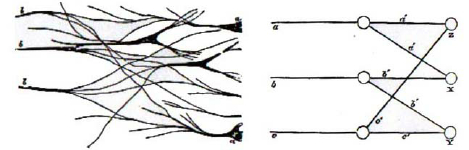
\includegraphics[scale=.7]{./images/bain.jpg}
\caption[From  \cite{bain1873mind}, pp. 110-111.]{From Bain's 1873 book \emph{Mind and Body}, which opens with the question ``What has Mind to do with brain substance, white and grey''?}
\label{bain}
\end{figure}

The notion that associations between thoughts and memories are based on neural connections in the brain was further developed in late 1800s by Sigmund Freud, who developed a psychodynamic theory, according to which  psychical ``energies'' are based on the flow of activations in the neural networks of the brain. His goal was to show how psychology could become a natural science by representing ``psychical processes as quantitatively determined states of specifiable material particles'' \cite[p. 355]{freud1954project}. But whereas earlier theorists had simply speculated about associative processes, he based his on actual  clinical observations, and in particular observations of (allegedly) neurotic patients experiencing ``excessively intense ideas.''  He explained his clinical observations in terms of ``neuronic excitation'' understood as ``quantities in a condition of flow'' (p. 356). Fig. \ref{freud} shows part of an image from this early book, which describes a patient (Emma Eckstein, who went on to become a famous author) who avoided shops based on an earlier traumatic experience. The specifics of the account are dubious, and Freud himself gave up on the project of a direct neural account of psychological processes,  but it does show that Freud was thinking about the mind in a broadly connectionist way.

\begin{figure}[h]
\centering
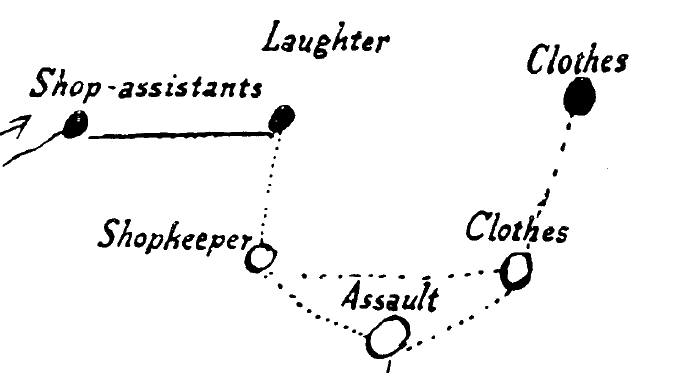
\includegraphics[width=0.5\textwidth]{images/freud_scientific_psychology.png}
\caption[From \cite{freud1954project}.]{An image from Freud's early \emph{Project for a Scientific Psychology}. The open circles are conscious ideas; the dark circles are unconscious ideas. }
\label{freud}
\end{figure}

% More on neuron doctrine, and how recent work may provide some limited support to Golgi? https://www.science.org/doi/10.1126/science.ade5645
Many other psychologists, neuroscientists, and philosophers in the late 19th and early 20th century contributed to the general idea that psychological processes are rooted in neural processes. Helmholtz, Mach, Ram{\'o}n y Cajal, Golgi, and others advanced biological psychology in various ways (see, e.g., \cite{boring1929history}), e.g. by establishing that neurons are individual cells, and by applying mathematical methods to psychology and neuroscience. In Russia, the psychologists Luria and Pavlov sought to understand the neural basis of associative learning, speech pathology, and other cognitive phenomena in a quantitative, experimentally tractable way.\footnote{On Luria in relation to the history of neural networks, see \cite[p. 41]{rumelhart1986parallel}.}

\section{Birth of Neural Networks}

We now turn to the history of neural networks proper, i.e. explicit formal descriptions of artificial neural networks, which could be implemented in computer programs.\footnote{The history of neural network research from this point forward is covered in several places. Fausett has a 4 page overview that covers the main points nicely:  \cite[pp. 22-26]{fausett1994fundamentals}. Levine, ch. 2 is especially detailed on McCulloch,s Pitts and Rosenblatt \cite{levine2000introduction}. A brief online history is at \url{http://cs.stanford.edu/people/eroberts/courses/soco/projects/neural-networks/History/}. A more recent history that extends to present day work in deep learning is at \url{https://www.skynettoday.com/overviews/neural-net-history}. Also see the end of chapter 1 of the first PDP chapter, \cite{rumelhart1986parallel}, and Haykin (2nd Ed.) section 1.9 \cite{haykin1998neural}. My favorite source is a series of interviews of leading figures in the history of neural networks collected in \emph{Talking Nets}, \cite{anderson2000talking}.} 

The first wave of research into neural networks occurred in the 1940s, via an array of neuroscientists, mathematicians, logicians, and engineers, many of them at MIT.\footnote{Important research relating to neural networks did occur earlier in the 20th century, e.g. work by Thorndike, Lashley, and Clark Hull. Hull's writings contain diagrams and formulas describing associative learning processes based on rat studies that look very much like connectionist networks (e.g. \url{http://psychclassics.yorku.ca/Hull/Hierarchy/part1.htm}).}   The history is complex, fascinating, and brimming with colorful personalities (see the early chapters of \cite{anderson2000talking}). This was the period when digital computers were first being developed by people like John von Neumann, a child prodigy who  later established a computer architecture still in use today (the ``von Neumann architecture'' \cite{von1981principles}). The architecture involves a separation between memory and a central processing unit that retrieves data from memory and operates on it using logical rules.
% Consider expanding the Hull discussion with a picture, esp. in light of the video

Neuroscience had also been steadily advancing in this period, and the network structure of the brain and its relation to behavior were better understood. The field of control theory was emerging via the work of Norbert Wiener, another child prodigy. He developed the field of ``cybernetics'' (which is closely related to modern control theory), and defined it as ``the science of control and communication in the animal and the machine'' \cite[p. 16]{wiener1948cybernetics}. In the late 1930s, the petroleum industry had developed central control systems to maintain refinery towers, and in WWII feedback systems were used to control anti-aircraft guns. A key idea in cybernetics was that these feedback circuits could coordinate complex movement, both in engineered systems and in the brain.

%  McCulloch: ``McCulloch was a psychiatrist and neuroanatomist by training: he spent some 20 years thinking about the representation of an event in the nervous system.
% Pitts. ```Pitt was a mathematical prodigy, who joined Mc Culloch in 1942.''
% They were logic oriented. Kleene had papers on this stuff. And these things emerged in the same literature as automata theory. Remember this is the beginning of formal logic and people realizing its potential.

In this atmosphere, two scientists emerged as the ``fathers of neural network theory'': Warren McCulloch (a neurophysiologist affiliated with cybernetics) and Walter Pitts (a logician).\footnote{Both had vivid personalities. McCulloch had wild hair and charisma. Pitts was a quiet introvert who had trouble getting a regular job, but who was regarded by his associates as a genius and was supported by McCulloch for many years. For a fascinating first-hand account of their personalities see the interviews with Lettvin, Cowan, and Arbib in \cite{anderson2000talking}. See in particular pages 9, 101, 104, 218, 223. Video interviews with McCulloch are available online.}  They wrote a famous paper  showing how neuron-like elements could perform all the logical operations performed by computers. This in turn implies that whatever can be done on a computer can, in principle, be done using neurons \cite{mcculloch1943logical}. A diagram from McCulloch and Pitt's famous paper, \emph{A Logical Calculus of Ideas Immanent in Nervous Activity}, is shown in figure \ref{mp}.\footnote{See Levine, p. 12, for a useful summary of how McCulloch / Pitts networks operate \cite{levine2000introduction}.}  In appendix \extref{ch_logicgates}, a demonstration of a similar approach to building logic gates using neural networks (in Simbrain) is developed.

\begin{figure}[h]
\centering
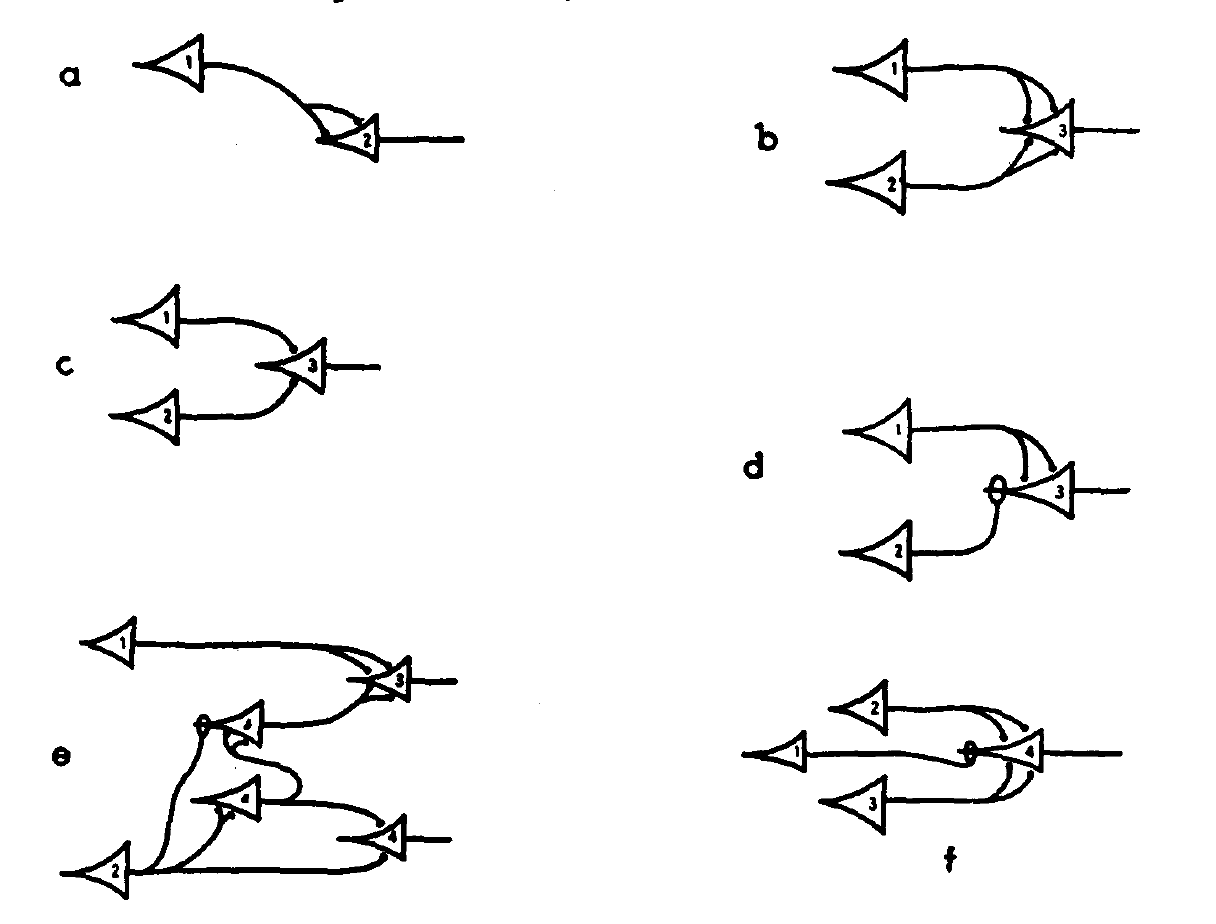
\includegraphics[width=0.5\textwidth]{./images/McCullochPitts.png}
\caption[From \cite{mcculloch1943logical}.]{From the end of McCulloch and Pitt's famous article, in which they demonstrate that ``for any logical expression satisfying certain conditions, one can find a net behaving in the fashion it describes.''  In these networks, what are today called ``weight strengths'' or ``synaptic efficacy'' correspond to number of connections. Nodes only fire if two or more incoming connections are activated. ``Lasso" connections correspond to what are today called ``inhibitory'' connections. In these networks, a single activated lasso connection will disable the node it is connected to. A network computing \emph{logical or} is shown in panel B (it will fire if either of the inputs nodes connected to it fires) and a network computing \emph{logical and} is shown in panel C (it only fires if both input nodes connected to it fire). Panel E models the heat illusion (briefly held cold objects can feel hot). For an elaboration of this case see \cite{piccinini2004first}.}
\label{mp}
\end{figure}
% Expand this. Explain the panel d is a connection with a shutoff, a bit like spiking 2 neurons and ch 1 ex.. Insert a reference to a Simbrain model of the heat illusion and include text from the video. // Maybe put labels in pic

McCulloch and Pitts used what are now called binary units or threshold units (see chapter \extref{ch_act_functions}): nodes that are only activated when their summed inputs are above a certain value. Nodes could only be active at a level of 0 or 1, based on the ``all or none'' property of neurons (cf. \extref{ch_neuro}). They made some assumptions that are unusual by today's standards. For example they assumed that a single inhibitory input is sufficient to completely prevent a neuron from firing. More importantly, they did \emph{not} describe connections between neurons using variable-strength weights. Their networks used fixed connections, which could not be adjusted using a learning rule. Learning rules would later become a  primary focus of neural network theorists. Nonetheless, it was the first time an actual formal model of a neuron was presented, together with a serious effort to understand how networks of neurons could produce complex behaviors.
% I think this is right, but check: \footnote{Though they did allow multiple connections between nodes, a multi-graph architecture not often used today.}

%Today neural networks are usually thought of in contrast to digital computers. In fact, in the introductory chapter \extref{ch_intro} we  opened by contrasting computation in a neural network with computation in a digital computer. But it is important to realize that this opposition came later. In this period people were just trying to figure out what a computer was. They were figuring out the mathematical underpinnings of computer science via the study of ``formal automata''. They knew the brain did some kind of computation and were interested in that. The neuroscientists were interested in what the logicians were doing. The engineers were interested in what the neuroscientists were doing. Etc. And in fact a neural network can implement a digital computer in principle. But in practice, the two styles of computation are distinct, and later on in the history the two approaches would be more strongly distinguished.

\section{The Cognitive Revolution}\label{cog_rev}

In the 1950s advances in linguistics, early computer science, neuroscience, and psychology, among others, coalesced in a broad reaction to earlier approaches to psychology, which had focused on observable behavioral data. The earlier \emph{behaviorists} had frowned upon discussions of internal processing between sensory inputs and motor outputs, and treated the mind as a kind of black box. The emerging cognitive scientists wanted to break open that black box and look inside: they wanted to understand what kind of processing occurs between sensory input and motor output in terms of \emph{computation}. The big idea that got everyone excited was that inside the mind there is an information processing system, one similar to the computer systems that were just then beginning to be realized on a large scale. This was sometimes referred to as the ``cognitive revolution'' in psychology.\footnote{An excellent overview and history of the era is \cite{baars1986cognitive}.}  

In the early cognitive revolution many different kinds of cognitive model were considered, including early neural networks like the Perceptron, discussed next. However, from early on there were doubts about neural networks. There were, for example, concerns that statistical approaches were fundamentally limited, a concern most famously posed by Minsky and Papert (see chapter \extref{ch_lms_backprop}). Others, were concerned that neural networks could not store and manipulate context-free symbols to use in reasoning \cite{fodor1988connectionism}, and there was also a worry that human-like language and reasoning could not be learned from the input stream used to train a neural network (``poverty of the stimulus'' arguments \cite{berwick2011poverty}). A competing approach to modeling cognition that avoided these problems was the symbolic approach---it goes by various names, including ``Symbolic AI'' and ``Classical AI''--according to which cognition involves manipulating symbols in accordance with rules (see section \extref{classicalAIComparison}). 

Over time, a kind of war broke out between these groups (brewing in the 1950s and peaking in the 1980s).  The connectionists had responded to the concerns raised by the symbolic AI camp, building networks that attempted to do all the things that symbolic AI advocates said they couldn't. The symbolic AI camp responded with doubts about these efforts, and for a time the ``framework wars'' were at the center of cognitive science. Today there are other camps as well, and some who mix ideas from both symbolic AI and connectionism. To jump ahead briefly, with the advent of large language models that produce convincing natural language, many feel that the Symbolic AI-connectionism war has been settled in connectionism's favor, and indeed  as noted in the introduction today ``AI'' is often used to refer to neural networks. But the symbolic approach has fought back against this, and in some sense the old debate has been rekindled (see section \extref{llmPhilosophy}).

Here are some themes in early cognitive science that prefigure connectionism. The Canadian psychologist and neuroscientist Donald Hebb formulated his famous learning rule for weights, the ``Hebb rule'' (``neurons that fire together, wire together'') \cite{hebb2005organization} (cf. the discussion of Hartley above).\footnote{See \url{http://www.scholarpedia.org/article/Donald_Olding_Hebb}. Also see Werbos' interview in  \cite{anderson2000talking}.}   Hebb also described the operation of the brain in terms of networks of connected neurons, formulating the concept of a ``cell assembly'', a group of neurons that becomes associated over time and thereafter tend to collectively reverberate in response to a stimulus (Fig. \ref{hebb} shows one of Hebb's own diagrams of a cell assembly) \cite{hebb2005organization}. The concept of a specific, learned pattern of brain activity produced by a stimulus remains important today.\footnote{See \url{http://www.scholarpedia.org/article/Cell_assemblies}. For a more up to date version of the idea cf. the concept of a polychronous neural group or PNG, \url{https://www.izhikevich.org/publications/spnet.htm}.}
% Need more information on the social network of Hebb. He does not seem too connected to the other figures.
% Some information in Haykin p. 38-39: ``Hebb's book was immensely influential among psychologists [like Anderson] but unfortunately it had little or no impact on the engineering community. Hebb's book [however] been the inspiration for the development of computational models of learning and adaptive systems" [Duda and Hart]   Uttley, leaky integrate and fire. 

\begin{figure}[h]
\centering
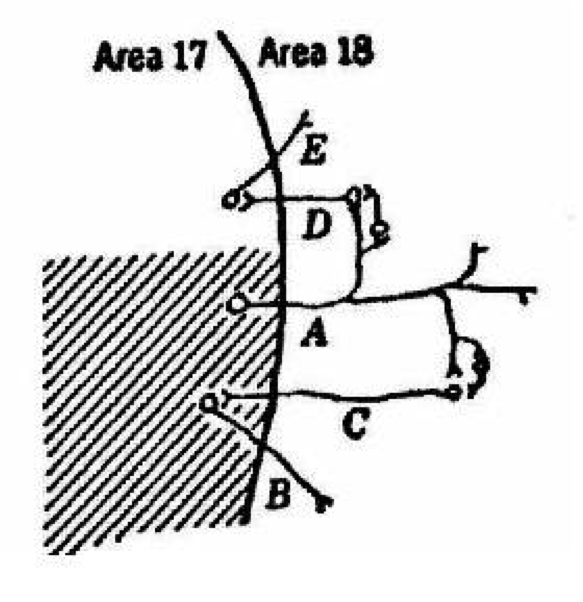
\includegraphics[width=0.4\textwidth]{./images/HebbCircuit.png}
\caption[From Hebb, 2005 \cite{hebb2005organization}]{A Hebbian cell assembly. These neurons initially fired together, and then got wired together, and so they will tend to fire together in the future.}
\label{hebb}
\end{figure}

\begin{figure}[h]
\centering
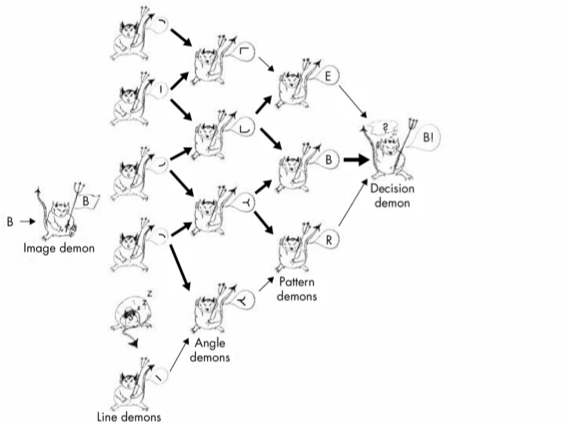
\includegraphics[width=0.5\textwidth]{./images/Selfridge.png}
\caption[From Groome, 2013 \cite{groome2013introduction}]{Selfridge's pandemonium model. Here the model is detecting the letter ``B''. The solid lines correspond to connections between active nodes, or ``demons''.}
\label{selfridge}
\end{figure}

Another important figure in the period was the psychologist Oliver Selfridge, who pioneered the idea that psychological processes can be broken down into interacting sub-processes. His ``Pandemonium'' theory described the mind as a collection of ``demons'', each of which takes care of one specific aspect of a task. For example, figure \ref{selfridge} shows how Selfridge thought of the process of perceiving the letter ``B''. As can be seen the figure, the demons are basically nodes and the model is basically a feed forward network. An image arrives at the eye, line demons detect lines and curves in various orientations, those demons send messages to the next layer of demons who detect combinations of lines and curves, etc. The process continues through a network of demons until a decision demon says ``B!'' \cite{selfridge1958pandemonium}.  This is a striking anticipation of the concept of a deep network for vision with layers of increasingly complex feature detectors (see chapter \extref{ch_cnn}).
% TODO: Add ref to 3b1b video 1, also video 2 at around 14:15 (https://youtu.be/IHZwWFHWa-w?list=PLZHQObOWTQDNU6R1_67000Dx_ZCJB-3pi&t=855)

%  Work here / add references
Other important research in this period was carried out by the psychiatrist and cyberneticist William Ashby (who wrote \emph{Design for a Brain} in 1952), Marvin Minsky (who wrote a dissertation on neural networks on 1954), and Dennis Gabor (a Nobel laureate who worked on holograms, and introduced a standard method for translating visual stimuli into a numeric form, that can be processed by neural networks).

\section{The Age of the Perceptron}\label{ageOfPerceptron}

The types of layered feed-forward networks that  are typically used today were first studied in detail in the 1950s and 1960s, primarily via the work of Frank Rosenblatt and Bernie Widrow (both published seminal papers in the late 1950s and early 1960s; see \cite{widrow1960adaptive}).\footnote{A concise summary of this period of history is in Bishop p. 98 \cite{bishop1995neural}. Also see \cite{widrow1960adaptive}.}  Rosenblatt called his network the ``Perceptron'' and Widrow called his an ``Adaline''. Both had a single layer of adjustable weights, threshold output units, and learned using an error function (see chapter \extref{ch_supervised}).Thus both networks moved beyond McCulloch and Pitt's networks---which did not involve any learning, just hand-crafted connections---to networks that actually learned from experience. This is, of course, what is distinctive about modern neural networks.

\begin{figure}[h]
\centering
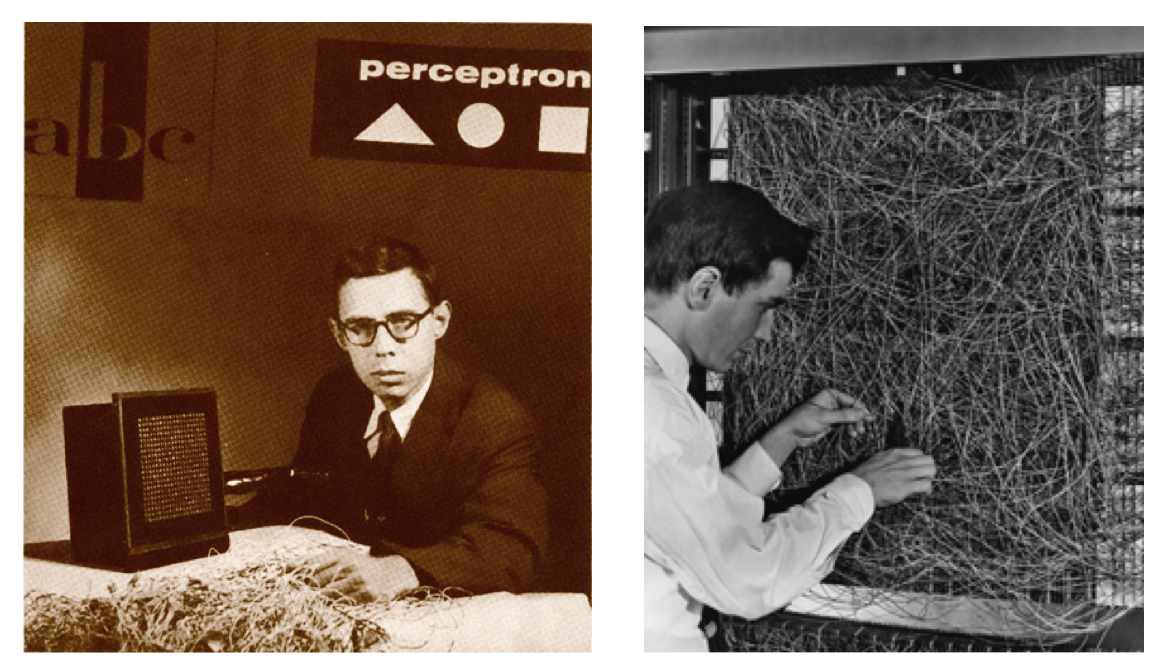
\includegraphics[width=0.7\textwidth]{images/perceptron.png}
\caption[Left: \url{http://www.rutherfordjournal.org/images/TAHC_rosenblatt-sepia.jpg}; Right: \url{http://www.newyorker.com/wp-content/uploads/2012/11/frank-rosenblatt-perception.jpg}]{Rosenblatt with one of his hardware implementations of a perceptron (left) and another view of the perceptron (right). }
\label{perceptron}
\end{figure}

Rosenblatt was a psychologist interested in human and animal behavior and its neural basis.\footnote{As with McCulloch and Pitts, Rosenblatt's personal history is fascinating, and in some ways tragic. See the Cowan and Hecht-Nielson interviews in Talking Nets \cite{anderson2000talking}.} He studied feed-forward networks with one layer of fixed weights and another layer of adjustable weights that could be trained to classify images on small displays as, for example, triangle vs. square, or male vs. female. He implemented his networks using huge tangles of wires for synaptic links (see Fig. \ref{perceptron}). This was quite impressive at the time and got a considerable amount of press.\footnote{See \url{https://www.youtube.com/watch?v=cNxadbrN_aI}} His rule was an early form of supervised learning rule based on a few if-then rules: if a sample is misclassified, then if output was too high, strengthen the weights, otherwise weaken the weights.  Rosenblatt proved that perceptrons could find solutions to certain types of classification tasks in a finite time \cite{rosenblatt1962comparison}.\footnote{This is known as the ``perceptron convergence theorem.'' For an intuitive discussion see \url{https://www.cs.cornell.edu/courses/cs4780/2018fa/lectures/lecturenote03.html}.} Haykin, who refers to this as the ``classical period of the perceptron'', summarizes Rosenblatt's importance as follows:
\begin{quotation}
The perceptron occupies a special place in the historical development of neural networks: It was the first algorithmically described neural network. Its invention by Rosenblatt, a psychologist, inspired engineers, physicists, and mathematicians alike to devote their research effort to different aspects of neural networks in the 1960s and the 1970s. Moreover, it is truly remarkable to find that the perceptron... is as valid today as it was in 1958 when Rosenblatt's paper on the perceptron was first published.
\end{quotation}
% Use the crazy Skynet quote about what Rosenblatt thought his machines would achieve

Whereas Rosenblatt focused on psychological implications of the perceptron, Widrow and his colleagues had engineering applications in mind, like adaptive noise cancelling in telephone wires.\footnote{According to Widrow this technology is used in every modem in the world and is at the heart of the internet; see \url{https://www.youtube.com/watch?v=skfNlwEbqck}. Widrow also implemented his networks using a special electrical components called a ``memistor'' which Widrow designed himself, which allowed weight updates in hardware. ALl of this is demonstrated in the video.} In the hardware implementation shown in Fig. \ref{adaline}, the toggle switches control input node activations, the knobs control weight strengths, and the dial shows the activation of an output node.\footnote{For Widrow's personal recounting of the Adaline and its history, see his interview in \emph{Talking Nets} \cite{anderson2000talking}. Also see the videos referenced in the figure caption, and the discussion in section \extref{lms_rule}}

\begin{figure}[h]
\centering
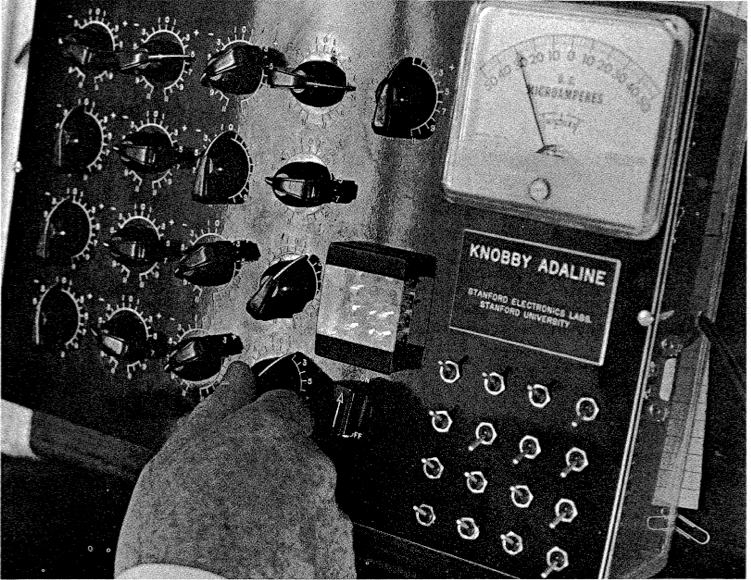
\includegraphics[scale=.3]{./images/adaline.png}
\caption[From \cite{widrow1963adaline}.]{A hardware implementation of Widrow and Hoff's ``Adaline'' network, which Widrow called the ``knobby Adaline'' on account of the prominent grid of knobs on the left, which control weight strengths, and which were manually adjusted to implement their learning algorithm. Inputs were produced using the 12 toggle switches on the lower right (and displayed in the grid of small lights), and the resulting output activation is displayed in the meter on the upper right. Videos of Widrow demonstrating the knobby Adaline, back in the 60s and also more recently, are available at \url{https://www.youtube.com/watch?v=skfNlwEbqck} and \url{https://www.youtube.com/watch?v=IEFRtz68m-8&t=161s}}
\label{adaline}
\end{figure}
% Show simbrain version

The least mean squares rule or LMS is discussed in section \extref{lms_rule}. Whereas Rosenblatt had derived his if-then rule from his understanding of biology, LMS was derived from calculus using first principles, which is how most modern learning rules are also derived. The essence of the rule is that we change each weight by a factor corresponding to the output error times the input node activation. This produces a kind of Goldilocks principle. When an output is too high (and the input is positive), we reduce the relevant weight so that the output will be lower, and  when an output is too low, we increase the relevant weight so that the output will be higher. In this way the network zooms in on the right value, so that the output is just right. This is, in a nutshell, the essence of how most modern neural networks work!  Widrow can be seen using this rule to train his machine to respond to T's and J's in variations positions in the video referenced in the figure caption. 

\section{The ``Dark Ages''}\label{dark_ages}

% Haykin points out the issues were part psychological, part financial. And other stuff. See p. 40
% Mention the convergence theorem itself
% Neocognitron, which anticipates deep learning. Done in industry. It's also a lot like pandemonium
% Sharai - We need references for Kohonen, Anderson, Braitenberg, Grossberg, and Carpenter.
% More on RL
% Compare the well-known AI winter, happened in another area but similar. Cf. Mitchell. Advised not to mention "AI" on her cv when she was on the market

Perceptrons and Adalines created a surge of interest in neural networks in the 1960s, but this was followed by a period of relative quiescence in the 1970s and 1980s, during what have been called the ``dark ages'', ``quiet years'', ``drought'', and ``winter'' of neural networks.\footnote{See PDP vol 1, ch. 1 \cite{rumelhart1986parallel}; Haykin p. 43 \cite{haykin1998neural}; Fausett p. 24 \cite{fausett1994fundamentals}. A variety of perspectives on the period are discussed in Talking Nets. 110, 155, 254, 305, 371. Grossberg, Carpenter, Kohonen, Anderson and others active in this period have their own interviews in Talking Nets \cite{anderson2000talking}.}  The dropoff in interest has been attributed to several causes. A key part of the story was that networks with a single layer of adjustable weights were shown by Minsky and Papert to suffer certain fundamental limitations \cite{minsky1969perceptrons} (see chapter \extref{ch_supervised}). So it was thought that neural networks weren't powerful enough to do psychologically realistic things. Moreover, at precisely that time more symbolic AI models were flourishing. 

However, even if interest in neural networks waned for a time, especially in comparison to AI, neural network research was active in this period. Relevant researchers include Kohonen, Fukushima, Anderson, Sutton, Barto, Braitenberg, Grossberg, and Carpenter. These and others laid the foundations for many of the ideas described in this book. So the dark years really weren't that dark.\footnote{Debates about the the status of neural networks in this period are covered in some detail in Talking Nets \cite{anderson2000talking}.} 
% Mention that Fukushima worked on early deep networks. Say a bit about the others too, at least in a footnote

\section{First Resurgence: Backprop and The PDP Group}\label{first_resurgence}

% This section needs to be enhanced. This is where we get the cog-sci stuff. It's what the book is supposed to be about. Refer back to Bain and Freud's hopes. This flashes by currently. OR at least refer back to the material in ch. 1 which does some of the work.

% See the connectionists email about the history of backprop, and all the discussion in talking nets. Clearly Werbos should be discussed, but there were others too.
% Sharai - We need a reference for the discovery of backpropagation algorithm (is discovery in reference to it's creation or it's first application in neural networks?).
Connectionism came out of its (allegedly) dark decade and enjoyed a resurgence in the 1980s, for several reasons. Prominent among these was the discovery of the backpropagation algorithm, which overcomes the limitations associated with perceptrons. This makes it possible train networks with more than one weight layer, which in turn allows them to solve more complex problems (for example, ``linearly inseparable'' classification tasks; see chapter \extref{ch_supervised}) by developing internal representations. A simple example of this is the ability to train a network to solve the exclusive or (XOR) logic gate. McCulloch and Pitts neurons could be hard-wired by hand to solve this problem, but no one could train a network automatically to solve it, because it requires an additional layer of processing. This is easy to see in Simbrain: you can easily build an XOR network by hand (appendix  \extref{ch_logicgates}), but try to use LMS to train a one weight layer network on the same problem and the error will never go to 0. 

The internal representations discovered in many-layered networks using backprop were shown to have important properties both for engineering applications and for psychological theories, as we will see throughout the book.\footnote{In future iterations we hope to expand this section with a summary of some of the major work that began in this era, primarily in connectionism, using neural networks to model psychological phenomena. As a first note in this direction, we refer to the table at the end of this paper: \url{https://link.springer.com/article/10.1007/s42113-020-00081-z/tables/1}.}

%The competing program of symbolic AI was running into problems \cite{dreyfus1992computers}. 

A related reason for this renewed interest---particularly among cognitive scientists---was the publication of a major two-volume work in the period, {\em Parallel Distributed Processing: Adventures in the Microstructure of Cognition}, in 1986, by David Rumelhart, James MClelland, and the ``PDP research group'' (a group of researchers, many of whom were at UC San Diego.)  This publication brought connectionist networks back to the forefront, by clearly articulating the connectionist standpoint, showcasing a number of models of various aspects of cognition, demonstrating how to interpret the internal states and representations of neural network models of cognition, and clarifying how connectionist networks differ from symbolic AI models \cite{rumelhart1986parallel}. John Hopfield's models of associative learning in recurrent networks (i.e. ``Hopfield nets'', discussed in chapter \extref{ch_unsupervised}) were also influential in this period, in part because Hopfield presented his work in an especially clear, mathematically precise way.\cite{hopfield1982neural}\footnote{In Talking nets, on the PDP group, see pp. 180, 254, 277, and 281. On  backprop and its history, see 286, 327, and 338. On Hopfield, see 113, 301 \cite{anderson2000talking}.}

% From Smolensky 1988: ``In the past half-decade the connectionist approach to cognitive modeling has grown from an obscure cult claiming a few true believers to a movement so vigorous that recent meetings of the Cognitive Science Society have begun to look like connectionist pep rallies''

% Net-talk was huge. See Talking Nets 324. I have material on this for other classes. Also Sejnowski is an important figure and should be mentioned.

\section{Second Decline and Second Resurgence: Convolutional Networks}\label{deep_revolution}

% Add reference to data science book that describes this sentiment. Maybe also that automatic diff video
For a time (roughly the late 1990s through about 2010), neural networks declined in interest as attention shifted to machine learning algorithms (cf. chapter \extref{ch_intro}). The problem was, in part, that tuning the parameters of a neural network seemed more an art than a science, especially when compared with machine learning, which is based on more tractable statistical principles. There was a sense that people just ``twiddled''  the knobs of a simulation as best they could until they got decent performance out of their network. In 2010 (in the midst of this decline), Phillip Jannert said: ``Neural networks were very popular for a while but have recently fallen out of favor somewhat. One reason is that the calculations required are more complicated than for other classifiers; another is that the whole concept is very \emph{ad hoc} and lacks a solid theoretical grounding'' \cite[Ch. 18]{janert2010data}.  There was a pervasive sense at the time that ``...neural nets were janky and did not work very well. They were seen as a hassle to work with---the computers were not fast enough, the algorithms were not smart enough, and people were not happy'' \cite{kurenkov2020briefhistory}.

However, several things happened that brought attention back to neural networks. First, larger datasets for training neural networks became available (what is sometimes referred to as ``big data''). Second, higher performance hardware for parallel neural network computing emerged, in particular using the graphical processing units or GPUs on graphics cards (the kinds used to play modern graphics intensive video games) and in proprietary hardware such as Google's tensor processing units (TMUs).\footnote{It is interesting that these games require lots of parallel processors to render texture and shading in real-time graphics processing using linear algebra (cf. chapter \extref{ch_linear_algebra}), and that the same parallel processing circuits can be used to run neural networks. When graphics cards were first developed they did not have neural networks in mind!} These breakthroughs suddenly allowed for the deployment of much larger \glossary{deep networks}. They not only had more layers, but relied on new, more complex, architectures.

Among these new architectures the most important were convolutional neural networks or CNNs (see   chapter \extref{ch_cnn}), which comprise sequences of convolutional layers, a special kind of weight layer in which a single set of shared weights is “scanned” over an input layer. Convolutional layers make it possible to effectively train deep networks with many more than 3 node layers.  CNNs led to an explosion of interest in deep learning and deep networks. Rather than only dealing with vectors and matrices, these architectures began to use more complex tensors (see \extref{sect_tensors}), such as ``volumes'' of activation describing images, videos, and other structures in rich detail.  Whereas most neural networks through the 1990s had just three simple node layers, CNN's can have tens or hundreds of layers, many of them multi-dimensional arrays. Thus networks with  a great deal of representational width and representational depth could be developed (see section \extref{structureNets} and chapter \extref{ch_cnn}). These many-layered convolutional networks existed as far back as the 1970s (via Fukushima's neocognitron and related models), but it is only in the 2010s  that a variety of technical hurdles relating to this type of network were surmounted. Indeed some have described the period beginning around the 2010s as a deep learning revolution, or as the decade of deep learning.\footnote{Andrey Kurenkov's history (\url{https://www.skynettoday.com/overviews/neural-net-history}) is excellent on these points. The achievements after 2010 are too numerous to survey here, but see \url{https://bmk.sh/2019/12/31/The-Decade-of-Deep-Learning/}.}  

\section{The Age of Generative AI}\label{age_generative_ai}

In 2017 Google introduced the \textbf{transformer architecture}---discussed in chapter \extref{ch_transformers}---which was subsequently adopted and extended by Open AI and many other groups in academia and industry \cite{vaswani2017attention}. The power of this architecture became widely known with the public release of Open AI's ChatGPT in 2022. ChatGPT had the fastest adoption rate of any software in history, and marked another shift in the history of neural networks and AI broadly. In this period, it became common to train extremely large models on vast amounts of data, using innovative new architectures like the transformer architecture. The resulting neural networks could be used to generate convincing outputs in multiple modalities, but especially text, video, and audio, hence the term \glossary{Generative AI}.\footnote{One mark of the shift is that it became extremely \emph{expensive} to train state-of-the-art models, and so reseachers could not train their own but had to rely on models trained by large companies such as Google, Open AI, and Microsoft.}$^,$\footnote{Though the term generative ``AI'' is used, this usually means \emph{neural networks} that have been used to generate these outputs, so this could more accurately be called ``generative neural networks'', but the term generative AI has stuck (see the first footnote in chapter \extref{ch_intro}).}

The transformer architecture builds on several streams of prior work. It is coming right off all the advances in training deep networks just discussed. They make use of huge datasets and benefit from innovations in hardware design.\footnote{As evidence, consider the explosive growth of NVIDIA, which started off in the graphics card business but is now a major driver of generative AI.} They develop many layers of internal representations that have a great deal of context awareness, which they can use to (for example) represent relationships between different parts of a fairly long conversation. The details are discussed in chapter \extref{ch_transformers}. The main initial use of transformer models was to generate natural language, and indeed ChatGPT is an example of a \glossary{large language model} (LLM), which is a language model trained on a large dataset--for example, a significant portion of text on the internet--to generate human-like text.\footnote{In fact, the terms ``transformer'' and ``llm'' have become conflated, though they are distinct (more on this in chapter \extref{ch_transformers}).}  The text produced by these models is now so convincing that they (in some contexts) pass the \glossary{Turing Test}, producing outputs that are not distinguishable from what a human can produce. Related advances (e.g. diffusion models) produce convincing images, videos and audio. 
% Matthew L: The interplay between the software and hardware innovations has been really cool to watch, with software (games) demanding certain kinds of hardware acceleration (GPUs), in turn enabling new kinds of software (large networks), causing new development in hardware (TPUs), in turn enabling bigger and more complex networks (transformers), that again then shaping the next generation of hardware (simpler operations with much higher parallelism and access to large amounts of memory with high bandwidth), in turn leading to... We'll see

These changes in the landscape of neural network research are significant enough that we are dubbing this the ``age of generative AI'' (the histories are just now being written, after all). This was when AI could really start generating new content, like news stories, essays, songs, images, and movies. In the future this will probably be seen as a landmark event, because this is when all the old doubts about neural networks were in a sense put to rest (of course, debate continues, but neural networks have clearly moved to the center of discussion), and when neural networks began to lead to fundamental changes in human existence, that we have not yet come to terms with.\footnote{This was also when ``artificial general intelligence'' (AGI) started entering the public consciousness, that is, AI that is not just able to do specific things in specific domains, but could behave in an intelligent manner in multiple domains and contexts. It is not generally believed AGI has been achieved as of yet.}

It has been a strange but exciting experience writing different versions of this chapter over the last few decades (the first version was written around 2005; see the Preface) as neural networks were out of vogue, then back in style, and then, arguably, completely transformed human society. No doubt more revisions to this chapter are coming, as the landscape continues to evolve.
